\chapter{Appendix}
\section{Appendix A}
\subsection{Backing up important data before uninstalling eSim}
\item Locate the folders : {\tt SubcircuitLibrary} and {\tt deviceModelLibrary} in the eSim installation directory, compress them in .zip or .rar format on your Desktop or some other location which does not contain eSim related files.
\item The projects created and stored in eSim-Workspace will not be deleted when one uninstalls eSim, hence there is no need to backup these project files. 
\item Newly created subcircuits and device models should be backed up as explained above. A way to take backup of the subcircuit blocks (external outlook) which appears in the schematic editor (not to be confused with internal circuit of the subcircuit) is explained in the Subcircuit section of this manual.

\subsection{Uninstalling eSim}

\subsubsection{For Windows OS users}
\item Locate the uninstaller {\tt "uninst-eSim.exe"} from the directory where eSim is present, by default it is installed at C:/FOSSEE/eSim/ 
\item Run the uninstaller executable and all the eSim related files and components \textbf{except} the projects created in \textbf{eSim-Workspace} will be deleted.

\subsubsection{For Ubuntu Linux OS users}
\item Open terminal and go to the location where eSim is stored using the cd command.
\item type the following and press enter : \\
\quad {\tt \$ ./install-eSim.sh --uninstall }
\section{Appendix B}

\subsection{Pin types in KiCad}


\begin{itemize}

\item {\textbf {Input}}: is a unidirectional input.
\item {\textbf {Output}}: is a unidirectional output that can drive high or low.
\item {\textbf {Bidirectional}}:can act as an input or an output. The I/O pins on microcontrollers are bidirectional.
\item {\textbf {Tri-state}}:is an output that can drive high or low, but can also be placed in a high-impedance state where it floats. The 74125 is a chip with tri-state outputs (sometimes called three-state outputs: high, low, and high-impedance).
\item {\textbf {Passive}}:is an unpowered connection, like resistors, capacitors and inductors.
\item {\textbf{Unspecified}}: is, unspecified. User would use that when no other classification fits.
\item {\textbf{Power input}}: is a pin where power comes in to a chip. Both the VCC and GND pins of chips would be classified as power inputs.
\item {\textbf {Power outputs}}: are where power comes out of a chip. The outputs of voltage regulators are the most common example of this pin type.
\item {\textbf {Open collector output}} pins: are outputs that can be driven low, but float 	otherwise. These are good for wired-AND connections where the output 	goes low if any of the attached open-collector pins goes low, but 	the output is pulled high by a pull-up resistor if all the pins are floating. The 7401 is a NAND gate chip with open-collector outputs.
\item {\textbf{Open emitter output pins}}: can be driven high, but float otherwise. These 	are good for wired-OR connections where the output goes high if any 	of the attached open-emitter pins goes high, but the output is pulled low by a pull-down resistor if all the pins are floating.
\item {\textbf{ Not-connected}}:pins are pins which have no function. Think of these as package pins that are not bonded to the IC inside.
 \end{itemize}

\subsection{ ERC Table}

     \begin{itemize}   

\item User can actually decide what you want to be told about, by setting the table below accordingly.For instance if the user wanted the ERC to throw an error if an input was connected to an input then the user would change the topmost box from green (no message) to yellow (warning) or red (error) as shown in \figref{erc_table} 

        \begin{figure}[!htp]
            \centering
            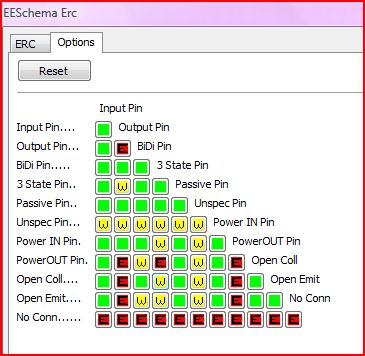
\includegraphics[width =\lgfig]{erctable.jpg}
            \caption{ERC Table}
         \end{figure}
\end {itemize}

  \section{Appendix C}
  \subsection{ Shortcut keys in Schematic editor }
     \begin {itemize}
\item Open the schematic editor and press Shift and ? keys simultaneously. This will display the total shortcut keys, also called as Hotkeys. Please note that, if the shortcut key is related to a component, for example, changing its value or its orientation etc, then your cursor must be located on that component.
\item {\textbf{V}}: This edits the Component’s value.
\item {\textbf{R}}: This rotates a component. 
\item{\textbf{A}}: This calls the place component tool through which you can add components in your schematic. 
\item{\textbf{M}}: This moves a component. After pressing M key, the component you chose will be tied to the cursor and you can place it anywhere in the schematic by clicking once on the schematic editor. 
\item{\textbf{C}}: This copies a component. After pressing C key, the component you chose will be tied to the cursor and you can place it anywhere in the schematic by clicking once on the schematic editor. 
\item{\textbf{Ctrl + H}}: This is to create a Global label. After pressing Ctrl + H keys simultaneously, the global label will be tied to the cursor and you can place it anywhere in the schematic by clicking once on the schematic editor. 
\item{\textbf{W}}: This calls the place wire tool through which you can add components in your schematic. 

\end {itemize}

\subsection{ Shortcut keys in PCB editor}

\begin {itemize}
\item The shortcuts that can be used in the Pcbnew Layout Editor .Open the Pcbnew Layout editor and press Shift and ? keys simultaneously.

\item {\textbf{X}}: This calls the Place Track tool. 
\item {\textbf{R}}: This rotates a component. 
\item{\textbf{B}}: Fill or Refill All Zones. 

\end {itemize}

\section {Appendix D: ERC errors}

\begin {itemize}

\item{\textbf{ErrType(1)}}: Duplicate sheet names within a given sheet.
Review sheet names in hierarchy and remove duplicates. 

\item{\textbf{ErrType(2)}}: Pin not connected and no No Connect Symbol.
Check the pin and wire overlaps or place No connect symbol if pin should be left unconnected.
 
\item{\textbf{ErrType(3)}}: Pin connected to some others pins but no pin to drive it.
This means there is a power input pin and there is no power connected to the pin. This is typically solved by adding a PWR FLAG symbol to the schematic.
 
\item{\textbf{ErrType(4)}}: Conflict problem between pins. Severity: warning.
Two pins connected but their function needs complementary signals (for ex. input -> output). You can have many power input pins connected to power output but no two power output pins should be connected together.

\item{\textbf{ErrType(5)}}: Conflict Problem between pins, Severity: Error. 
This is because you can only have one output or power output on the same net. 

\item{\textbf{ErrType(6)}}: Mismatch between hierarchical labels and pins sheets. 
There is a mismatch between hierarchical label and existing pin sheet, try to re-import hierarchical pins to replace wrong pin sheet. 

\item{\textbf{ErrType(7)}}: A no connect symbol is connected to more than 1 pin. 
"No connect" symbol should be put at the end of the pin,and this pin should be left unconnected at all costs.

\item{\textbf{ErrType(8)}}: Global label not connected to any other global label. 
There is a global label which has no pair in other sheet(s). 

\item{\textbf{ErrType(9)}}: Two labels are equal for case insensitive comparisons 
Review schematic labels to find possible duplicates, watch for similarity of large and small letters. 

\item{\textbf{ErrType(10)}}: Two global labels are equal for case insensitive comparisons. 
Review global labels in hierarchy to find possible duplicates, watch for similarity of large and small letters.

\end {itemize}
\pagebreak

\section {Appendix E: Checks to be done before Simulation in NGHDL}
\begin{compactenum}
\item VHDL filename should be in small letters without any space or special characters (Underscore is allowed).
\item Entity name, architecture declaration and the VHDL file name should match exactly.
\item Declaration of each port should be done on a new line. See \textbf{nghdl/Example/} for further reference.
\item Port declaration can be either \textbf{std\_logic} or \textbf{std\_logic\_vector}. No other declarations are allowed.
\item All \textbf{in} ports should be declared before \textbf{out} ports.
\item Maximum number of output ports that a VHDL entity under simulation can have is 64, provided the port names are not too lengthy to overflow the buffer.
\item Be extremely careful while dealing with Arithmetic Operations. \\ 
(See \textbf{nghdl/Example/counter/counter.vhdl} for further reference)
\item If structural style is used, then the main entity of your VHDL code which is to be simulated,  should be declared first in the file with inclusion of libraries for subsequent declaration of each supporting entity.
See \textbf{nghdl/Example/full\_adder/ \\ full\_adder\_structural.vhdl} for further reference.
\item Do not use \texttt{sudo} or root permissions while working Mixed-Mode Simulation and eSim.
\item If there are more than one VHDL file to be uploaded, then do it \textbf{one-by-one}, as described below:
    \begin{compactenum}
    \item Click on \texttt{NGHDL} button on eSim or type \texttt{nghdl}/ in terminal. A new window will be opened.
    \item Upload your first VHDL file and wait for the process to be completed.
    \item Check if there are any Errors on the console. If possible, try to debug it and report 
        your error and its solution to us. Otherwise, you can send the error to us. If there are no errors, upload your second model and repeat the steps mentioned above. \\
        You can upload as many models as required.
    \end{compactenum}
\item \textbf{Do not upload two or more VHDL files simultaneously :}    \\
\texttt{Add files} option allow you to use a smaller entity / subpart / submodule to support the main VHDL file. That is, a digital model will be generated corresponding to that file that has been browsed. The file that has been \texttt{added} to Nghdl upload window will only be placed along with the model under model’s DUTghdl folder to support the model.

Hence, \texttt{browsing} one file and \texttt{adding} several files won’t create that many number models, but only model will be created corresponding to the browsed file.
\item Maximum number of NGHDL models that can be simulated at once is restricted to 512.
\item Next simulation should be started only after the completion of the previous/current  simulation. No two simulations should be executed at once.
\item While providing parameters to the adc-dac bridges that correspond to any NGHDL model, make sure that the \textbf{rise and fall delays of ADC and DAC bridges} are comparable to the simulation time parameters passed. Some examples are given below: \\
        \begin{compactenum}
        \item \textbf{Circuits involving both Analog and NGHDL Components} - If step time is 10 ms and simulation time is 200 ms, then DAC-ADC delays should be atleast 1 us.
        \item \textbf{Circuits involving only NGHDL Components} - If step time is 10 ms and simulation time is 200 ms, then DAC-ADC delays should be atleast 500 us.
        \item \textbfCMOS inverter subcircuit [INVCMOS] has a delay of 6 ms(can be changed by changing capacitor value inside the CMOS subcircuit). 
        NGHDL model created, ADC and DAC bridges has rise and fall time 1 ns. You are simulating this circuit for 100 ms, it won’t work. Increase the rise and fall delay for the ADC-DAC models from 1 nanosecond to 1 microsecond (1/1000th of the analog delay).
        \end{compactenum}
        
        In general \textbf{(a thumb rule to follow)}, delay value can be set to at least 1/500th part of the stop time.
\item If there is a need to use multiple instances of same NGHDL model in a given project and if even one of these instances need to have a different parameter value than the rest of the instances, then a separate NGHDL model needs to be generated with a different name.
\end{compactenum}

\pagebreak 

\section {Appendix F: Common Errors in NGHDL}

Before concluding anything about NGHDL’s working or about eSim’s Mixed-Mode Simulation, do check the console for outputs and logs. Kindly see the following errors on User’s end that can be rectified there itself :

\subsection{NGHDL Upload Errors}

\begin{itemize}
    \item \textbf{Error while opening NGHDL. Please make sure NGHDL is installed :}

 \\
As the error indicates, NGHDL is not installed at all or there has been some error during installation which was not resolved effectively. However, if the installation was done correctly, then open a terminal and type : \\

\noindent \texttt{\$ sudo ln -s <your\_path\_to\_nghdl>/nghdl/src/ngspice\_ghdl.py /usr/loc\linebreak     al/bin/nghdl}


Now type  \texttt{nghdl} in terminal and check if the \texttt{NGHDL Digital Model Creator} window opens or not.

\item \textbf{Error - select a *.vhdl file :} \\
This type of error can occur due to a variety of underlying user issues. Check terminal from which eSim is launched for more detailed errors. However, following is a list of common mistakes that a user may face : 
\begin{itemize}
    \item \texttt{Permission Denied} - Change the permission of \texttt{ngspice-nghdl} folder 
recursively to be used by all the users. To do so, open a terminal and type:
\begin{center}
    \texttt{\$ sudo chown \$USER:\$USER -R \$HOME/ngspice-nghdl/}
\end{center} 

\end{itemize}

%\item \textbf{Re-uploading *.vhdl file: }\\
    %\begin{itemsize}
 %    In this case, if one tries to re-upload a *.vhdl file that has already been processed through NGHDL before, and one misplaces or deleted the ifspec.ifs file of that model from the DUT directory, an error is inevitable.
  %  \begin{center}
   %     \texttt{If one must make changes to the vhdl code once already processed, please edit the *.vhdl file under DUTghdl/ directory of that particular model instead of re-uploading.}
    %\end{center}
   % \end{itemsize}


\end{itemize}

\subsection{Simulation Related Errors}

\begin{itemize}
    \item \textbf{GHDL compilation error : }\\
The VHDL code itself is incorrect, as a result the corresponding model generated is incorrect and no simulation will be done. Kindly upload a correct VHDL code. 

\item \textbf{Warning : There is an 'U'$\vert$'X'$\vert$'W'$\vert$'Z'$\vert$'-' in an arithmetic operand, the result will be 'X'(es) : }\\
Such warnings are difficult to find in xterm outputs. However, it indicates that there is some logical error in your VHDL code regarding the data types / arithmetic operations / type conversions, etc. Kindly upload a logically correct VHDL code.

\item \textbf{Unknown model name $\langle$your\_nghdl\_model$\rangle$ - Ngspice : } \\
If this error occurs on xterm window while simulating with Ngspice, then check whether the Ngspice engine used is of system built or that of the NGHDL. To check the same, follow the steps:
\begin{enumerate}
    \item Open terminal and type : \texttt{\$ whereis ngspice}
    \item Go to the location where ngspice executable is found.
    \item Now, check if this ngspice is a link to: \\ \texttt{ngspice-nghdl/install\_dir/bin/ngspice}
    \item If it is not a link, then uninstall the system’s installed ngspice and create a link 
to the above mentioned path by typing the command in terminal as:

\texttt{\$ sudo ln -s \$HOME/ngspice-nghdl/install\_dir/bin/ngspice/<previo\linebreak us\_ngpsice\_location>/ngspice}
\item If output of step 1 is empty, then run above command by replacing\linebreak \texttt{<previous\_ngpsice\_location>} with \texttt{/usr/bin}
\end{enumerate}

\item \textbf{Unknown model name $\langle$your\_nghdl\_model$\rangle$ - KiCad-to-Ngspice : }

If this error occurs during KiCad-to-Ngspice conversion, then check whether the uploaded VHDL file had any Uppercase characters or any other special characters in its filename. Note that only lowercase characters and underscores are allowed.

\item \textbf{Warning : component instance \texttt{uut} of \texttt{xyz}  is not bound  : }

This logical error is related to the VHDL code which is shown as a Warning and simulation plots may also appear. However, these plots are incorrect as the VHDL model itself is incorrect. 
Following are the examples that can cause this error:
\begin{itemize}
\item If a vhdl file is saved as \texttt{dummycode.vhdl} and the entity and architecture 
are declared as for example, \texttt{codedummy} or \texttt{dummy} or something other than the name of the actual vhdl file itself, one will get the above error.
\item If structural style is being used and above error is seen, then kindly make the necessary changes by referring our example found at:\\ \texttt{nghdl/Example/full\_adder/full\_adder\_structural.vhdl}
\end{itemize}\\
Kindly check with the GHDL documentation and online resources too are available regarding this GHDL error.

\item \textbf{Warning : Too many analog/event-driven solution alternations \\
     Warning : Convergence problems at node (net-*). \\         
            ………………………. \\
     Transient solution failed - \\
     doAnalyses: iteration limit reached : } 

As the error says itself that if too many analog components are connected to digital model due to which there can be many analog alternations (or if too many events are generated rapidly due to which the convergence would fail for those models), then the initial conditions won’t converge and the transient solution will fail. Follow these steps to resolve it:
\begin{enumerate}
    \item Open the corresponding project’s cir.out file \texttt{(“*.cir.out”)}.
    \item Just below the \textbf{“.control”} statement and above the \textbf{“run”} statement, insert a new 
     line.
     \item On this new line, type \textbf{“option noopalter”}.
     \item Save the file and exit.
     \item Run the simulation once again.
\end{enumerate}


\item \textbf{doAnalyses: TRAN : Timestep too small; time = ... , timestep = …; 
       trouble with node ... 
       run simulation(s) aborted :}

As the error says :
\begin{itemize}
    \item Check if the time-step is too small as compared to the stop-time. 
    \item If the time-step is of the same order(scalable) as that of the stop-time, then check the delays of the adc-dac bridges and make them comparable to simulation stop-time.
    \item If the delays are comparable, then check the parameters provided to the digital and analog models  and set them appropriately.
\end{itemize}

\item \textbf{chmod : changing permissions of ‘any\_file’: Operation not permitted : }

This error, displayed on xterm by Ngspice, is similar to that of \texttt{Permission Denied} error. Kindly refer \textbf{section 13.4.1} for the same.
\end{itemize}

\subsection{Model Deletion}

If you want to delete a model from your file system or is deleted due to unavoidable circumstances, perform the following steps (to ensure consistency within the software) :
\begin{enumerate}
    \item Delete the folders found at path :
    \begin{itemize}
        \begin{itemize}
        \item
        \texttt{ngspice-nghdl/src/xspice/icm/ghdl/<your\_model>/} 
        \item \texttt{ngspice-nghdl/release/src/xspice/icm/ghdl/<your\_model>/}
        \end{itemize}
    \end{itemize}
    \item Delete the name and description of that model from the files :
    \begin{itemize}
        \begin{itemize}
        \item
     \texttt{ngspice-nghdl/src/xspice/icm/ghdl/modpath.lst}
     \item  \texttt{eSim\_Nghdl.lib}
     \end{itemize}
    \end{itemize}
    
     Realign the content of these files by            removing any extra spaces or empty lines found between any two subsequent remaining         model names after deletion.
    
    \item Delete the file found at path : \\
    \texttt{eSim-version/src/modelParamXML/Nghdl/<your\_model>.xml}
    
\section {Appendix G: References}
\item [1] A. S. Sedra and K. C. Smith, Microelectronic Circuits - Theory and Applications. Oxford University Press, 2009. 
\item [2] K. M. Moudgalya, “Spoken Tutorial: A Collaborative and Scalable Education Technology,” CSI Communications, vol. 35, no. 6, pp. 10–12, September 2011, available at https://spoken-tutorial.org/CSI.pdf. 
\item [3] (2020, March). [Online]. Available: https://www.scilab.org/ 
\item [4] (2020, March). [Online].
Available: https://scilab-test.garudaindia.in/scilab\_in/ \\
https://scilab-test.garudaindia.in/cloud 
\item [6]  K. Kannan and K. Narayanan, “Ict-enabled scalable workshops for engineering college teachers in india,” in Post-Secondary Education and Technology: A Global Perspective on Opportunities and Obstacles to Development (International and Development Education), R. Clohey, S. Austin-Li, and J. C. Weldman, Eds. Palgrave Macmillan, 2012. 
\item [7]  (2020, March). [Online]. Available: https://esim.fossee.in 
\item [8] (2020, March). [Online]. Available: http://www.aakashlabs.org/ 
\item [9] (2020, March). [Online]. \\
Available: http://en.wikipedia.org/wiki/Electronic\_design\_automation
\item [10] (2020, March) Synaptic Package Manager Spoken Tutorial. [Online]. Available: https://www.spoken-tutorial.org/tutorial-search/?search\_foss=Linux&search\_language=English 
\item [11] (2020, March). [Online]. Available: https://www.kicad-pcb.org/
\item [12] (2020, March). [Online]. Available: ngspice.sourceforge.net/
\item [13] (2020, March). [Online]. Available: http://scilab.in/ 
\item [14]   S. M. Sandler and C. Hymowitz, SPICE Circuit Handbook. New York: McGraw-Hill Professional, 2006. 
\item [15]   J.-P. Charras and F. Tappero. (2020, March). [Online]. Available: https://docs.kicad-pcb.org/
\item [16] Wayne Stambaugh (2020, March). [Online]. \\
Available: https://launchpad.net/kicad/4.0/4.0.7 
\item   [17]   P. Nenzi and H. Vogt. (2020) Ngspice users manual version 31. [Online]. \\
Available: http://ngspice.sourceforge.net/docs/ngspice-manual.pdf 
\item [18]   K. M. Moudgalya, “LATEX Training through Spoken Tutorials,” TUGboat, vol. 32, no. 3, pp. 251–257, 2011. 
\item [19]   (2020, March). [Online]. Available: https://www.spoken-tutorial.org/ 
\end{enumerate}
